\documentclass[a4paper,12pt]{article}

\usepackage[utf8]{inputenc}
\usepackage{graphicx}
\usepackage{color}
\usepackage{amsmath}
\usepackage{amsthm}
\usepackage{amssymb}
\usepackage{array}
\newcolumntype{L}{>{$}l<{$}}
\newcolumntype{C}{>{$}c<{$}}
\newcolumntype{R}{>{$}r<{$}}
\usepackage[text={14.0cm,21.0cm}]{geometry}
\usepackage{rotating}
\usepackage{hyperref}
\usepackage{caption}
\usepackage{subcaption}
\usepackage{algorithm}
\usepackage[noend]{algpseudocode}
\usepackage[indention=18pt]{subcaption}
\theoremstyle{definition}
\newtheorem{vb}{Voorbeeld}[subsection]
\newtheorem{vbn}{Voorbeelden}[subsection]
\newtheorem{definition}{Definitie}[subsection]
\newtheorem{opm}{Opmerking}[subsection]
\newtheorem{eig}{Eigenschap}[subsection]
\newtheorem{eign}{Eigenschappen}[subsection]
\newtheorem{st}{Stelling}[subsection]
\newtheorem{lem}{Lemma}[subsection]
\renewcommand*{\proofname}{Bewijs}
\renewcommand*{\figurename}{Figuur}
\renewcommand*{\tablename}{Tabel}
\renewcommand*{\contentsname}{Inhoudsopgave}
\renewcommand*{\refname}{Bibliografie}
\newcommand{\SSE}{\text{SSE}}
\newcommand{\CSSE}{\text{SSE}_{cluster}}
\newcommand{\SSB}{\text{SSB}}
\newcommand{\TSSB}{\text{SSB}_{total}}
\newcommand{\TSS}{\text{TSS}}
\newcommand{\pushcode}[1][0]{\item[]\hskip\dimexpr#1\algorithmicindent\relax}

\makeatletter
\renewcommand{\ALG@name}{Algoritme}
\def\BState{\State\hskip-\ALG@thistlm}
\makeatother

%%%%%%%%%%%%
% niet aanpassen
\makeatletter
\newcommand\faculteit[1]{\newcommand\@faculteit{#1}}
\newcommand\vakgroep[1]{\newcommand\@vakgroep{#1}}
\newcommand\promotor[1]{\newcommand\@promotor{#1}}
\renewcommand*{\maketitle}{
	\thispagestyle{empty}
	\begin{center}
	
\includegraphics[width=\textwidth]{logobalk_ugent.pdf}

	\vspace{1cm}
	\huge \@faculteit

	\LARGE \@vakgroep

	\vfill{\Huge\textbf\@title}

	\vspace{1.5cm}{\Huge\textbf\@author}

	\vspace{3cm}\LARGE Promotor: \@promotor\vfill

	\Large Bachelorproef ingediend tot het behalen van de academische graad van bachelor in de Wiskunde.

	\vspace{1.5cm}\@date
	\end{center}
\clearpage}
\makeatother

%%%%%%%%%%%%
% wel aanpassen
\title{Clusteringsalgoritmen}
\author{Victor Miclotte}
\date{Academiejaar 2015--2016}
\promotor{Prof.\ Dr.\ V.\ Fack}
\faculteit{Faculteit Wetenschappen}
\vakgroep{Vakgroep Toegepaste Wiskunde}
%%%%%%%%%%%%


\begin{document}
\pagenumbering{gobble}
\newgeometry{top=20mm,bottom=30mm,left=20mm,right=20mm}% kies zelf je marges
\maketitle
\newpage
\pagenumbering{arabic}
\section*{Dankwoord}
Ik wil graag enkele mensen bedanken voor de bijdrage die ze geleverd hebben aan
dit werk. Eerst en vooral gaat mijn dank uit naar mijn promotor prof. dr. Veerle
Fack voor het voorstellen van het interessante onderwerp en de begeleiding met
relevante feedback.\\
\ \\
Daarnaast wil ik mijn ouders en broer bedanken voor het 
nalezen van dit werk, mij te wijzen op taalkundige fouten en ook op vlak van
layout interessante feedback te geven.\\
\ \\
Tot slot wil ik mijn kotgenoten en vrienden
bedanken om geïnteresseerd te luisteren naar wat ik over mijn werk te vertellen had
en ook om voor de nodige afleiding te zorgen.

\newpage
\tableofcontents
\newpage
\setcounter{section}{0}
\section{Inleiding}

Clustering is het verdelen van data in groepen (clusters), zodanig dat data in
dezelfde cluster meer verwant zijn aan elkaar dan aan data uit andere clusters.
Er is geen unieke ideale manier van clusteren, bijgevolg is er geen universele
clusteringsmethode maar bestaan er veel verschillende algoritmen.
Deze kunnen totaal verschillend zijn, afhankelijk van de notie van clusters en
hoe deze worden gezocht. Meestal wil men een cluster waarvoor
de datapunten (de elementen van de cluster) dicht bij elkaar liggen, of met een hoge
densiteit. Er is geen standaard `beste' algoritme om data te clusteren,
elk algoritme heeft zijn plus- en minpunten en zal beter of slechter presteren
dan een ander algoritme afhankelijk van de gegeven dataset.
In dit werk zullen we de basis van clustering, enkele veelgebruikte algoritmen
en toepassingen bespreken.
We beginnen met het bespreken van enkele definities en manieren om data voor te
stellen. Vervolgens bespreken we drie basisalgoritmen om data te clusteren, de 
plus- en minpunten van de algoritmen zullen besproken worden. In 
Sectie~\ref{sec:eval} worden enkele manieren gegeven om de kwaliteit van een
clustering na te gaan. Tot slot bespreken we kort enkele toepassingen van 
clusteringsalgoritmen.\\
\ \\
Clustering wordt in heel veel takken van de wetenschap gebruikt, 
vaak zal men bij het analyseren van data vooraf de data proberen te groeperen zodat
er geen appels met peren vergeleken worden. Het vinden van belangrijke of interessante
tekstdocumenten kan ook gebeuren m.b.v. clusteringsalgoritmen. Men kan op voorhand
een aantal teksten klasseren en dan bepalen tot welke categorie nieuwe teksten
behoren door een clusteringsalgoritme te gebruiken. Ook in de bio-informatica
worden clusteringsalgoritmen volop gebruikt, bijvoorbeeld bij het analyseren
van microarrays om expressies van bepaalde genen te proberen achterhalen.
Niet alle mensen reageren op dezelfde manier op bepaalde medicatie, soms zal
een medicijn bijvoorbeeld een positief effect hebben op de ene persoon maar geen
of zelfs een negatief effect op een andere persoon. Door de evolutie van het maken
en het analyseren van microarrays, zal men mis\-schien ooit medicijnen kunnen voorschrijven
die aangepast zijn aan het genexpressieprofiel van de patiënt.

\newpage
\section{Data representatie en definities}

Om clusteringsalgoritmen en hun resultaten goed te kunnen begrijpen is het cruciaal
dat men data correct kan interpreteren en verbanden zoals afstanden tussen
datapunten kan definiëren. In veel gevallen is het mogelijk om data voor te stellen
in een $d$-dimensionale euclidische ruimte.

\subsection{Pattern matrix}
We beschouwen een dataset bestaande uit $n$ gegevens die elk $d$ attributen (metingen)
hebben. Deze data kan voorgesteld worden door $n$ vectoren in een $d$-dimensionale 
ruimte, of nog, als een $n \times d$ ``pattern matrix''. Elke rij in deze matrix
stelt een datapunt voor en elke kolom een attribuut.



\subsection{Afstandsmatrix en gelijkheidsmatrix}
\label{sec_proxmat}
Om data te kunnen clusteren moet er een notie van afstand of associatie tussen
de datapunten zijn. Hiervoor definiëren we een dichtheidsindex:

\begin{definition}
 Een dichtheidsindex is een functie
 $d: U \times U \subseteq \mathbb{R}^d \times \mathbb{R}^d \rightarrow \mathbb{R}$
 waarvoor:
 \begin{itemize}
  \item $d(i,i) = 0\  \forall i \hspace{50pt}$ (identiteit),
  \item $d(i,k) = d(k,i)\  \forall i,k \hspace{10pt}$ (symmetrie),
  \item $d(i,k) \geq 0\  \forall i,k \hspace{35pt}$ (niet-negativiteit).
 \end{itemize}
\end{definition}

\begin{opm}
 Deze definitie geldt voor data die voorgesteld kan worden in een $d$-dimensio\-nale
 euclidische ruimte. Men spreekt van een metriek (of afstand) als in het 
 bijzonder ook voldaan is aan $d(i,k) \leq d(i,j) + d(j,k)\ \forall i,j,k$ (driehoeksongelijkheid) 
 en $d(i,k) = 0 \Leftrightarrow i = k$ (scheidingseigenschap).
\end{opm}

Met behulp van vorige definitie definiëren we nu een afstandsmatrix. Deze matrix
zal de enige vereiste input zijn voor een clusteringsalgoritme, we zullen echter vaak nog de afstandsmatrix
moeten berekenen indien enkel de ruwe data (pattern matrix) gegeven is. Dit is altijd mogelijk eenmaal een
afstand gedefinieerd is, het omgekeerde zal in het algemeen niet mogelijk zijn.

\begin{definition}
 Een afstandsmatrix voor een verzameling van $n$ $d$-dimensionale datapunten
 ${x_1, ..., x_n}$ is een $n\times n$ symmetrische matrix $(d_{i,j})$ met
 $d_{i,j} = d(x_i, x_j)$ waarbij $d(\cdot,\cdot)$ een dichtheids\-index is.
\end{definition}


\begin{vb}
 Hier zijn enkele voorbeelden van metrieken. Beschouw punten $x$ en $y$ $\in \mathbb{R}^d$.
 \begin{enumerate}
  \item[(i)] Minkowski afstand (L$_p$-norm): $d(x,y) = \left(\sum\limits_{i=1}^d|x_i-y_i|^p\right)^{\frac{1}{p}}$ met $p\geq1$
  \item[(ii)] Manhattan afstand (L$_1$-norm): $d(x,y) = \sum\limits_{i=1}^d|x_i-y_i|$
  \item[(iii)] Euclidische afstand  (L$_2$-norm): $d(x,y) = \sqrt{(x_1-y_1)^2 + (x_2-y_2)^2 + ... + (x_d-y_d)^2}$
  \item[(iv)] Supremum afstand  (L$_\infty$-norm): $d(x,y) = \max\limits_{1\leq i\leq d}|x_i - y_i|$
 \end{enumerate}
\end{vb}

Een andere manier om data voor te stellen, is door gebruik te maken van een gelijkheids\-matrix.
Een gelijkheidsmatrix $(a_{i,j})$ wordt analoog gedefinieerd, $a_{i,j}$ stelt in dit geval de `gelijk\-heid' tussen
het $i$-de en het $j$-de datapunt voor.

\begin{definition}
 Een gelijkheid is een functie
 $s: U \times U \subseteq \mathbb{R}^d \times \mathbb{R}^d \rightarrow [0,1]$ met 
 $s(x,y) = 1$ als $x$ en $y$ `gelijk' zijn
 en $s(x,y)=0$ als $x$ en $y$ totaal verschillend zijn. 
\end{definition}

\subsection{Normalisatie en projectie}
Soms is ruwe data niet geschikt voor clustering. Bijvoorbeeld als één attribuut
in mijl is geschaald en een ander in meter, dan zal de tweede meting veel meer
invloed hebben dan de eerste als men de euclidische afstand gebruikt. Daarom is
er vaak nood aan normalisatie van de data (bijvoorbeeld d.m.v. herschaling)
vooraleer men de data kan clusteren.

\ \\
Om een beeld te krijgen van de data (na clustering) zijn lineaire projecties zeer
handig. Vaak zullen de datapunten meerdimensionale vectoren zijn die niet visueel
voor te stellen zijn. Door de data te projecteren op een ruimte van lagere dimensie
(2 of 3) kunnen we als mens een beter zicht krijgen op de gevormde clusters.


\subsection{Soorten clusteringen en clusters}
We voeren nu enkele definities in die verschillende soorten
clusteringen van elkaar onderscheiden.
\begin{definition}
\item
 \begin{itemize}
  \item \textbf{Partitioneel clusteren:} het resultaat van de clustering is een
	partitie van de data, i.e. elk datapunt zit in precies één cluster.
  \item \textbf{Hiërarchisch clusteren:} het resultaat van de clustering is een
	geneste opeenvolging van partities (elk element van een partitie is een
	deelverzameling van een element van de volgende partitie in de sequentie).
  \item \textbf{Exclusief clusteren:} elk datapunt behoort tot exact één cluster.
  \item \textbf{Overlappend clusteren:} een datapunt kan tot meerdere clusters behoren.
  \item \textbf{Fuzzy clusteren:} elk datapunt behoort tot elke cluster met een
	bepaald gewicht tussen 0 en 1. Vaak wordt een extra voorwaarde opgelegd,
	namelijk dat de gewichten per datapunt optellen tot 1.
  \item \textbf{Compleet clusteren:} elk datapunt behoort tot minstens 1 cluster.
  \item \textbf{Partieel clusteren:} niet elk datapunt hoeft tot een cluster te 
	behoren, dit is voornamelijk van toepassing in geval van outliers.
 \end{itemize}
\end{definition}

\begin{opm}
Theoretisch gezien is partitioneel clusteren zeer eenvoudig. Omdat er slechts een
eindig aantal datapunten beschouwd worden, kan men alle mogelijke clusteringen bepalen.
Dan hoeft men enkel maar te kijken welke van deze clusteringen het best voldoet aan
het vooropgestelde criterium dat bepaalt of een clustering goed is. Het is natuurlijk
duidelijk dat dit enkel theoretisch zal werken, vaak is de hoeveelheid data zodanig
groot dat dit te veel rekenwerk en geheugen zou vereisen om nuttig te zijn.
Het aantal mogelijke clusteringen van $n$ objecten in $k$ niet lege clusters
wordt gegeven door de Stirling getallen van de tweede soort
$S(n,k)$
(Appendix~\ref{stirling}).
\end{opm}


Omdat de kwaliteit van een cluster afhangt van wat het doel is van de clustering,
zijn er verschillende mogelijkheden om `goede' clusters te bekomen. Daarom 
definiëren we enkele soorten clusters.

\begin{definition}
\item
 \begin{itemize}
  \item \textbf{Goed gescheiden clusters:} elk datapunt in een cluster ligt dichter bij
	elk ander datapunt in de cluster dan bij een datapunt buiten de cluster.
  \item \textbf{Prototype-gebaseerde clusters:} elk datapunt in een cluster ligt
	dichter bij het `prototype' van de cluster dan bij een `prototype' van
	een andere cluster. Dit `prototype' is een centraal gelegen
	punt van de cluster, vaak het zwaartepunt.
  \item \textbf{Graaf-gebaseerde clusters:} data worden voorgesteld d.m.v. een
	graaf, een cluster is meestal een component van de graaf, i.e. een verzameling
	toppen die een samenhangende graaf vormen. Men kan ook clusters zien als klieken,
	i.e. complete componenten.
  \item \textbf{Dichtste-buur clusters:} elk datapunt behoort tot dezelfde
	cluster als zijn dichtste buur.
  \item \textbf{Dichtheid-gebaseerde clusters:} een cluster is een `dichte' verzameling
	van datapunten, omgeven door een strook met lage densiteit.
 \end{itemize}

\end{definition}

\newpage
\section{$k$-means}
\label{sec_kmeans}
Een veelgebruikt algoritme om data te clusteren is het $k$-means algoritme.
In deze sectie zullen we ons verdiepen in het algoritme zelf, de correctheid en
de voor- en nadelen ervan. $k$-means is een prototype-gebaseerde clusteringstechniek.
Dit algoritme leent zich het best voor data die beschreven kan worden in een
$d$-dimensionale Euclidische ruimte. De prototypes van de clusters stemmen overeen
met de centers.

Een gelijkaardig algoritme 'K-medoid' zal in plaats van centers werken met
medoids, een medoid is het meest representatieve punt van een cluster. In
tegenstelling tot een center zal dit altijd een datapunt zijn, terwijl
centers over het algemeen geen datapunten zullen zijn.

\subsection{Algoritme}


Gegeven een dataset met $n$ elementen zal het $k$-means
algoritme een partitie van $k$ deelverzamelingen vormen.
$k$-means is een iteratief algoritme, eerst worden er $k$ initiële centers gekozen. Deze zullen
iteratief aangepast worden tot ze niet meer veranderen.
Dat gebeurt als volgt: eerst worden alle datapunten aan de cluster met het dichtste
center toegevoegd, daarna worden de centers van alle clusters opnieuw
berekend en wordt de procedure herhaald.

\begin{algorithm}
\caption{$k$-means}\label{kmeans}
\textbf{Input:} een verzameling $\{x_1, \ldots, x_n\}$ $d$-dimensionale datapunten en een getal $k$.\\
\textbf{Output:} een verzameling $\{c_1, \ldots, c_k\}$ centers van clusters.
\begin{algorithmic}[1]
\State Kies $\{c_1, \ldots, c_k\} \subseteq \{x_1, \ldots, x_n\}$ als initiële
centers.
\While{$\{c_1, \ldots, c_k\}$ is veranderd}
\State Maak $k$ clusters door elk datapunt toe te voegen aan de cluster met het dichtste center.
\State Herbereken de centers van alle clusters en pas $\{c_1, \ldots, c_k\}$ aan.
\EndWhile
\end{algorithmic}
\end{algorithm}

Dit algoritme zal niet altijd convergeren naar een oplossing, convergentie
hangt in dit geval af van de definitie van de afstandsfunctie en een center.
Omdat de convergentie in de eerste iteraties veel sterker is dan in de latere
iteraties, wordt de voorwaarde op lijn~2 van algoritme~\ref{kmeans} vaak
vervangen door een zwakkere voorwaarde (bijvoorbeeld: minder dan $1\%$ van de
datapunten is veranderd van cluster).

Het iteratieve deel van het basis $k$-means algoritme bestaat uit twee delen: het toekennen
van datapunten aan een cluster (met dichtstbijzijnde center) en het herberekenen van
de centers. Om punten aan de correcte cluster toe te voegen, moet er een goed gedefinieerde
notie van afstand zijn. De meest gebruikte afstanden zijn de Euclidische afstand
(voor data in een Euclidische ruimte) en de cosinusgelijkenis
\footnote{De cosinusgelijkenis ($d(u,v) = \dfrac{u\cdot v}{\|u\|\|v\|}$ met 
$u$ en $v$ vectoren) wordt voornamelijk gebruikt om gelijkenis van twee 
tekstdocumenten te beschrijven, de waarden van de vectoren stellen dan de 
frequentie van een bepaalde term/woord voor.}. Er zijn echter alternatieven 
die specifiek nuttig blijken voor bepaalde data. Zo kan de Manhattan afstand gebruikt 
worden voor Euclidische data en de Jaccard afstand voor tekstdocumenten. Omdat in 
het algoritme veel afstanden worden berekend, wordt
meestal een eenvoudig te berekenen afstand gebruikt. Soms is het mogelijk door gebruik te 
maken van de onderliggende structuur waarin de data zich bevindt (bvb. een 
Euclidische ruimte van lage dimensie) om het aantal afstanden die berekend worden 
te beperken en zo het algoritme te versnellen. In Sectie~\ref{bisect} bespreken we 
nog een andere manier om het aantal berekeningen te beperken.

Het herberekenen van de centers van de clusters maakt gebruik van een
doelfunctie en de reeds gedefinieerde afstandsfunctie. Deze doelfunctie kan 
bijvoorbeeld het minimaliseren van de som van de kwadratische Euclidische
afstanden (SSE, sum of squared errors) van de punten tot de centers
zijn voor Euclidische data, of het maximaliseren van de cosinusgelijkenissen 
tussen de punten en centers voor tekstdocumenten.
In Figuur~\ref{fig:kmeans} wordt een visualisatie van het $k$-means algoritme gegeven.


\begin{figure}[!ht]
    \centering
    \begin{subfigure}[t]{0.3\textwidth}
        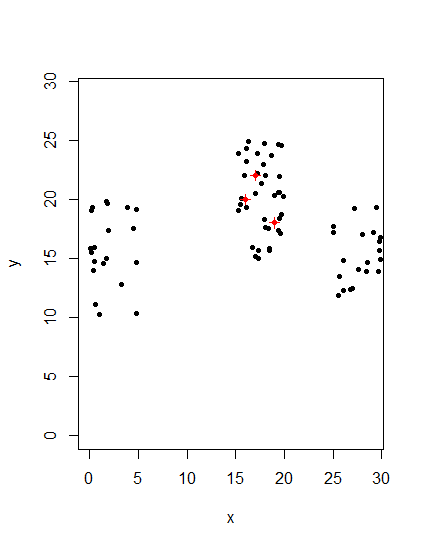
\includegraphics[width=\textwidth]{kmeans.png}
        \caption{De data met initiële centers in het rood.}
    \end{subfigure}
    \begin{subfigure}[t]{0.3\textwidth}
        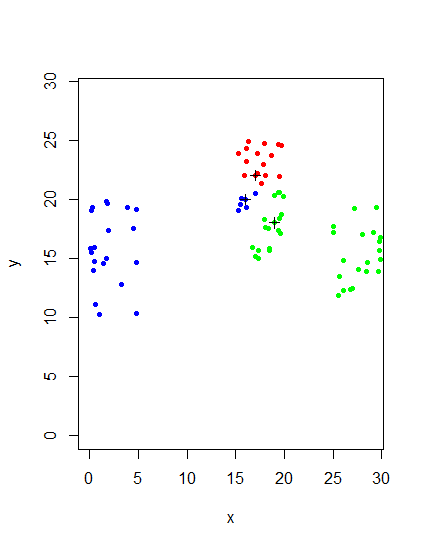
\includegraphics[width=\textwidth]{kmeans_it0.png}
        \caption{De datapunten worden geclusterd naargelang het dichtste center.}
    \end{subfigure}
    \begin{subfigure}[t]{0.3\textwidth}
        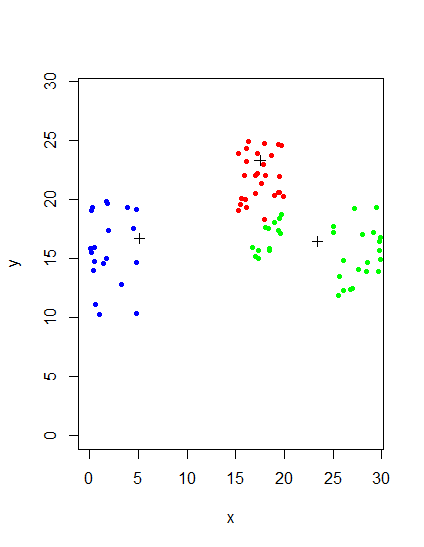
\includegraphics[width=\textwidth]{kmeans_it1.png}
        \caption{De centers worden herberekend en de punten worden opnieuw geclusterd.}
    \end{subfigure}
    \begin{subfigure}[t]{0.3\textwidth}
        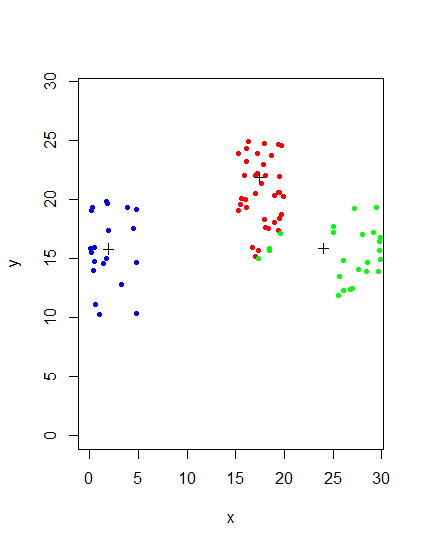
\includegraphics[width=\textwidth]{kmeans_it2.png}
        \caption{De centers worden herberekend en de punten worden opnieuw geclusterd.}
    \end{subfigure}
    \begin{subfigure}[t]{0.3\textwidth}
        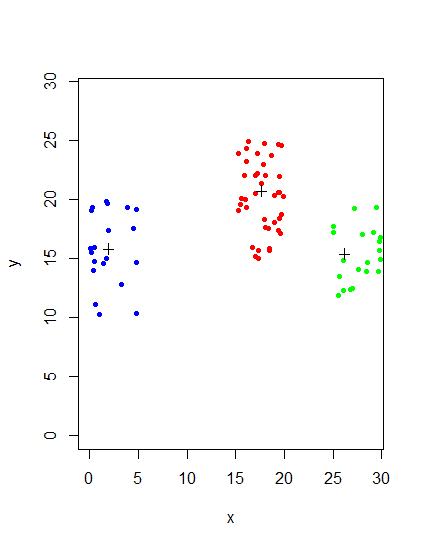
\includegraphics[width=\textwidth]{kmeans_it3.png}
        \caption{De centers worden herberekend en de punten worden opnieuw geclusterd.}
    \end{subfigure}
    \begin{subfigure}[t]{0.3\textwidth}
        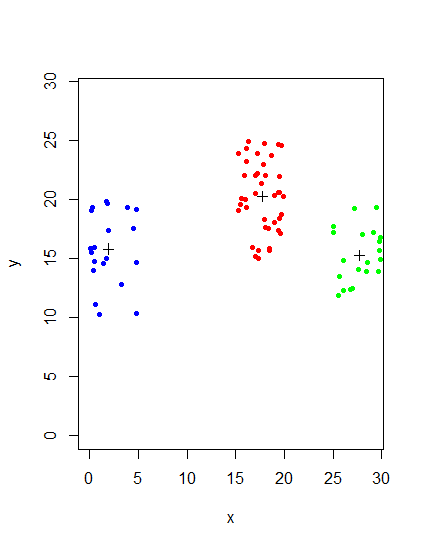
\includegraphics[width=\textwidth]{kmeans_it4.png}
        \caption{De centers worden herberekend en de punten worden opnieuw geclusterd,
        de clusters blijven ongewijzigd, het algoritme is voltooid.}
    \end{subfigure}
    \caption{Visualisatie van het $k$-means clusteringsalgoritme.}\label{fig:kmeans}
\end{figure}


\subsection{Sum of Squared Errors: SSE}
\label{SSE}
In vele gevallen zullen we Euclidische data beschouwen met daarbij de Euclidische
afstand als afstandsmaat. Om de kwaliteit van een clustering na te gaan, zal men
veelal gebruik maken van de som van de kwadratische afstanden tussen de punten
en hun bijhorende zwaartepunten, dit noemt men de Sum of Squared Errors (SSE).
De ``error'' van een punt is gedefinieerd door de afstand van dat punt tot het
dichtstbijzijnde zwaartepunt.

\begin{st}
 Het center van een cluster dat de SSE minimaliseert, wordt gegeven door
 het Euclidische zwaartepunt van de cluster.
\end{st}

\begin{proof}
 We geven hier het bewijs voor het eendimensionale geval, het geval voor $n$ dimensies is volledig
 analoog.
 
 De Sum of Squared Errors (in één dimensie) wordt gegeven door:
 $$\SSE=\sum\limits_{i=1}^k\sum\limits_{x\in C_i}(c_i - x)^2.$$
 Waarbij $C_i$ de $i$-de cluster is met $c_i$ als center en $x$ een punt van
 $C_i$. Om het $k$-de center te bepalen waarvoor de SSE minimaal wordt,
 leiden we de SSE af naar $c_k$ en stellen we het resultaat gelijk aan nul.
 \begin{align*}
  0 &=  \dfrac{\partial \SSE}{\partial c_k}\\
  &= \dfrac{\partial}{\partial c_k}
  \sum\limits_{i=1}^k\sum\limits_{x\in C_i}(c_i - x)^2\\
  &= \sum\limits_{i=1}^k\sum\limits_{x\in C_i}\dfrac{\partial}{\partial c_k}
  (c_i - x)^2\\
  &= \sum\limits_{x\in C_k}2(c_k - x) = 
  2\left(m_kc_k-\sum\limits_{x\in C_k}x\right), \quad \text{met } m_k = |C_k|.\\
 \end{align*}
We vinden $c_k =
\dfrac{1}{m_k}\sum\limits_{x\in C_k}x$ en $c_k$ is dus het Euclidisch zwaartepunt
(of gemiddelde) van de cluster $C_k$.
\end{proof}


\subsection{Problemen}

\subsubsection{Initiële centers}
Een andere belangrijke stap die het resultaat van de clustering zwaar zal 
beïnvloeden, is het kiezen van de initiële centers. Het is eenvoudig in 
te zien dat als men per toeval initiële centers kiest die dicht bij de eigenlijke 
centers liggen, dit in het algemeen een beter resultaat (of sneller een resultaat)
geeft dan wanneer men de initiële centers kiest die in één en dezelfde
finale cluster liggen. 
Om deze reden wordt het algoritme vaak meermaals uitgevoerd op dezelfde data maar 
met verschillende beginsituaties, waarna de beste clustering geselecteerd wordt.

Het is echter ook mogelijk om in plaats van willekeurige beginsituaties te 
beschouwen, de initiële centers zodanig te kiezen dat er een grotere kans is
op een betere clustering. Zo kan men bijvoorbeeld meer dan $k$ initiële 
centers selecteren en vervolgens uit die punten de $k$ selecteren die het 
meest verspreid liggen. Een gelijkaardige methode selecteert de initiële 
centers één voor één door telkens het verste datapunt toe te voegen 
(het eerste center wordt willekeurig gekozen). Het is makkelijk in te zien 
dat de bekomen centers goed verspreid zullen liggen, wat in het algemeen 
beter zal zijn dan een willekeurige selectie van punten. Het bepalen van deze 
punten vereist echter extra rekenwerk en is gevoelig voor outliers. Beide problemen 
kunnen grotendeels vermeden worden door de methode toe te passen op een sample van 
de data in plaats van de hele dataset. Outliers zijn uitzonderingen in de data en 
komen dus slechts in kleine mate voor. De kans dat ze voorkomen in de sample is 
dus eerder klein, terwijl de kans dat een punt van een dicht gebied in de sample 
voorkomt veel groter is. Er zal ook veel minder rekenwerk vereist zijn om de 
verste punten in de kleine sample te berekenen. 

Een andere manier om een betere beginsituatie te vinden, maakt gebruik van de
hiërarchisch clustering methode die we bespreken in Sectie~\ref{hierarch}.
Een sample van de volledige dataset wordt hiërarchisch geclusterd en vervolgens 
worden de centers berekend van de gevonden clustering met $k$ clusters. 
De gevonden centers zullen dan net de initiële centers voor het $k$-means algoritme
zijn. Deze methode is effectief maar vergt veel rekenwerk en is daarom vooral nuttig
voor kleine datasets.
In Figuur~\ref{fig:kmeans_bad} zien we hoe een slechte beginsituatie een totaal
verkeerd beeld van de clusters kan bekomen.

 \begin{figure}[!ht]\centering
  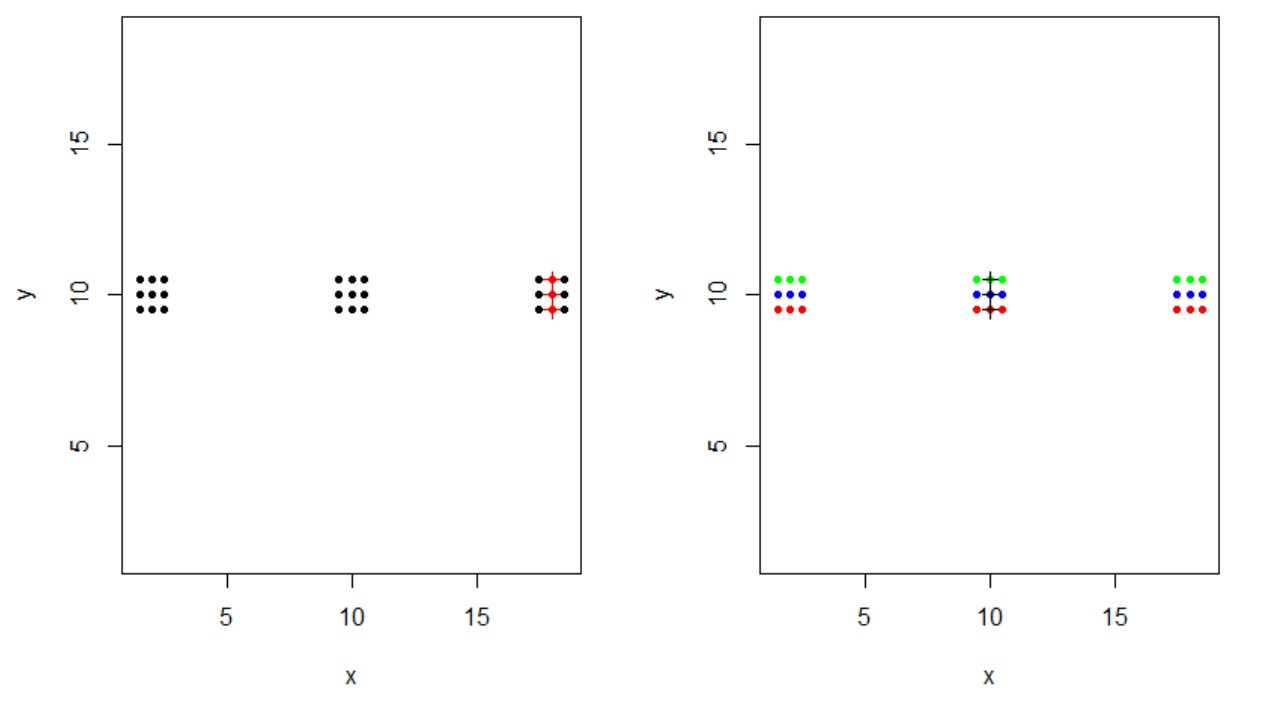
\includegraphics[width=10cm]{kmeans_bad.jpeg}
  \caption{Visualisatie $k$-means clusteringsalgoritme met een slechte beginsituatie.}
  \label{fig:kmeans_bad}
 \end{figure}

\begin{opm}
In het geval dat de initiële centers zodanig gekozen worden dat er net in
elke effectieve cluster één ligt, zal de kans op succes in het algemeen hoger zijn.
De kans dat dit gebeurt wanneer de beginsituatie willekeurig gekozen wordt, is
echter klein voor grote $k$: $$P = \dfrac{\text{aantal manieren om uit elke
cluster één center te selecteren}}{\text{aantal manieren om $k$ clusters te
selecteren}} = \dfrac{k!n^k}{(kn)^k} = \dfrac{k!}{k^k}.$$ Voor $k=10$ is die kans
slechts $10!/10^{10} = 0.00036$.


 \begin{figure}[!ht]\centering
  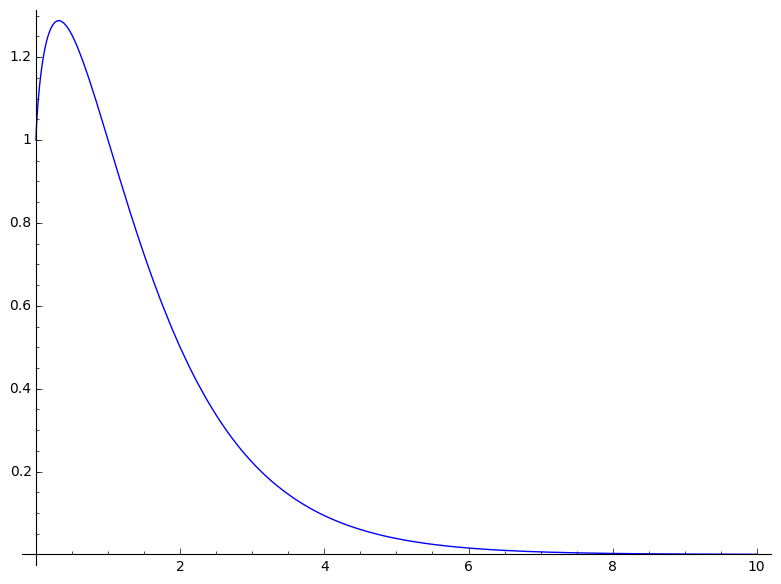
\includegraphics[width=10cm]{kans_plot.png}
  \caption{Plot van $\dfrac{k!}{k^k}$, de kans convergeert snel naar $0$.}
  \label{fig:kmeans_bad}
 \end{figure}
 
\end{opm}

\newpage
\subsubsection{Lege clusters}
Omdat de centers van clusters geen datapunten hoeven te zijn, is het mogelijk
dat er lege clusters ontstaan. Als dit het geval is, zal de
clustering niet optimaal zijn en kan deze gemakkelijk aangepast worden om
een beter resultaat te verkrijgen.
Men kan dit oplossen door het center van de lege cluster te verwijderen en
een nieuw center te zoeken, bijvoorbeeld door het verste punt te nemen (let
op: ook hier kunnen outliers een grote invloed hebben op het resultaat). Men kan
ook een center nemen uit de cluster met de slechtste score en zo deze cluster in
twee opsplitsen en de score verbeteren. In geval van meerdere lege clusters
kan men dit meermaals herhalen tot alle clusters niet leeg zijn.

\subsubsection{Speciale soorten clusters}
Zolang de clusters sferisch zijn en ongeveer gelijke densiteit en groottes hebben,
presteert het $k$-means algoritme vrij goed. Wanneer men echter speciale soorten
clusters heeft, zal het $k$-means algoritme vaak geen goed resultaat leveren. Dit probleem
kan tegengegaan worden als men tevreden is met subclusters. Als men een voldoende groot
aantal clusters op voorhand specificeert, zullen de gevormde clusters meestal
subclusters zijn van de eigenlijke clusters.

\subsection{Uitbreidingen}
Er bestaan heel wat uitbreidingen die voor specifieke data beter werken
dan het basis $k$-means algoritme. Uitbreidingen kunnen bijvoorbeeld de data
vooraf aanpassen (pre-processing), het resultaat van het basisalgoritme verbeteren
(post-processing),  of een variatie op het basisalgoritme
zijn. In deze sectie bespreken we enkele van deze uitbreidingen.

\subsubsection{Post-processing: verlagen van de SSE}
Zoals we eerder al hebben opgemerkt, is het minimaliseren van de SSE een populaire
methode om een goede clustering te bekomen voor Euclidische data. Een clustering
bekomen door het basis $k$-means algoritme zal typisch convergeren naar een lokaal
minimum voor de SSE. Omdat het globaal minimum in het algemeen lager ligt,
willen we de bekomen clustering verbeteren en een lagere SSE 
bekomen. Men zou kunnen het aantal clusters vergroten en zo eenvoudig de SSE
verlagen, maar meestal is dit niet het doel. Liever zouden we een lagere SSE bekomen
zonder het aantal clusters aan te passen. De totale SSE wordt gegeven door de som van
de SSE van elke cluster. Om dit te verlagen, moeten we dus de SSE van clusters apart
verlagen. Dit gebeurt in twee fasen: $(1)$ het aantal clusters verhogen
om de SSE te verlagen en $(2)$ het samenvoegen van clusters waarbij de SSE zo weinig
mogelijk toeneemt. Door te alterneren tussen beide fasen is het mogelijk om een 
lokaal minimum te verlaten en een andere clustering te bekomen.

In de eerste fase kan men bijvoorbeeld een cluster opsplitsen, hiervoor wordt meestal
de cluster genomen met hoogste SSE. Een alternatief is om een nieuw center
te maken, men neemt hiervoor meestal het punt dat het verste ligt van alle andere
centers. Merk op dat dit rekenintensief is, tenzij de errors van alle datapunten
worden bijgehouden, wat geheugenintensief is.

Het samenvoegen van clusters kan gebeuren door een cluster weg te nemen, i.e. het center
wordt verwijderd en de datapunten van de cluster worden aan andere clusters toegevoegd.
Het is duidelijk dat men hier clusters verkiest met lage SSE om de toename te beperken.
Een andere manier is het samenvoegen (merge) van twee clusters zodat de toename in
SSE zo laag mogelijk is, deze methode wordt ook gebruikt bij het hiërarchisch
clusteren in Sectie~\ref{hierarch}.

\subsubsection{Bisecting $k$-means}
\label{bisect}
Het bisecting $k$-means algoritme maakt gebruik van het 
basis $k$-means algoritme om een partitionele $k$-clustering, i.e. een clustering
bestaande uit $k$ clusters, te bekomen. Het algoritme vertrekt van één cluster die
alle datapunten bevat. In elke stap wordt één van de clusters gesplitst en 
dit wordt herhaald tot er $k$ clusters zijn.

\begin{algorithm}
\caption{Bisecting $k$-means}\label{bisectalgo}
\textbf{Input:} een verzameling $\{x_1, \ldots, x_n\}$ $d$-dimensionale datapunten.\\
\textbf{Output:} een lijst $C = \{c_1, \ldots, c_k\}$ clusters.
\begin{algorithmic}[1]
\State Initialiseer $C$ met één cluster die alle punten bevat.
\While{$|C| < k$}
\State Verwijder een cluster $c_j$ uit de lijst.
\State Splits $c_j$ op een vooraf bepaald aantal ($n$) manieren in twee delen.
\For{$i = 1$ to $n$}
\State $k$-means$(c_j, k = 2)$.
\EndFor
\State Bepaal de beste clustering (van de $n$ bekomen clusteringen van $c_j$).
\State Voeg de twee clusters bekomen door deze clustering toe aan de lijst van clusters.
\EndWhile
\end{algorithmic}
\end{algorithm}

Het selecteren van de cluster die gesplitst wordt, kan op verschillende 
manieren gebeuren. Men kan kiezen voor de cluster met de hoogste SSE of de cluster
met het grootste aantal punten, of men bepaalt de cluster aan de hand van een
criterium dat gebruik maakt van beide. De bekomen clustering is, in tegenstelling
tot een clustering bekomen door het basisalgoritme, in het algemeen geen lokaal
minimum voor de SSE. Het basisalgoritme wordt lokaal gebruikt om een cluster in twee
delen te splitsen. Om deze reden worden de centers van de bekomen
clusters vaak gebruikt als beginsituatie voor een finale uitvoering van het basisalgoritme.



\newpage
\section{Hiërarchisch clusteren}
\label{hierarch}
In deze sectie zullen we een ander belangrijk clusteringsalgoritme bespreken:
hiërarchisch clusteren. We onderscheiden twee soorten hiërarchische clustering methoden:
\begin{itemize}
 \item \textbf{Agglomerative (bottom up):} men start van een situatie waar elk
 datapunt een cluster is, clusters worden per twee samengevoegd totdat er één
 triviale cluster overblijft die alle datapunten bevat.
 \item \textbf{Divisive (top down):} men start met één cluster die alle datapunten
 bevat en verdeelt die recursief totdat elk datapunt in een aparte cluster ligt.
\end{itemize}

De agglomeratieve methode wordt veruit het meest gebruikt van de twee, we zullen
ons dus vooral toespitsen op dit algoritme en de term ``agglomeratief'' achterwege
laten. Hiërarchische clusteringen worden
voornamelijk voorgesteld met behulp van een dendrogram (Figuur~\ref{fig:dendrogram}). Dit is een boomdiagram
waarin de clusters met hun subclusters zichtbaar zijn en waaruit men duidelijk
de volgorde van het samenvoegen van clusters kan aflezen.
In het speciale geval van $2$-dimensionale data kan men gebruik maken van een
genest clusterdiagram. De voorstelling m.b.v. een dendrogram zal veel frequenter
voorkomen omdat er geen voorwaarde op de data wordt opgelegd in tegenstelling tot
de voorstelling m.b.v. een genest clusterdiagram.

 \begin{figure}[!ht]\centering
  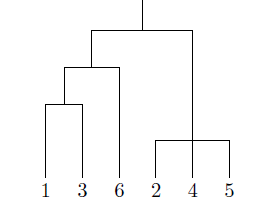
\includegraphics[width=7cm]{dendrogram.png}
  \caption{Een dendrogram: gebruikt voor het visualiseren van een hiërarchische clustering.
   De bladeren van de boom stellen datapunten voor, clusters worden systematisch samengevoegd
   totdat er uiteindelijk één cluster overblijft in de wortel.}
  \label{fig:dendrogram}
 \end{figure}
 
 
\subsection{Algoritme}
Gegeven een dataset van $n$ datapunten, zal een hiërarchisch clusteringsalgoritme
een sequentie van partitionele clusteringen bekomen met volgende eigenschappen:
\begin{enumerate}
 \item De eerste partitionele clustering is de partitie bestaande uit $n$ singletons.
 \item Elke element van een partitionele clustering zal een deelverzameling zijn van
 een element van de volgende partitionele clustering in de sequentie.
 \item De sequentie bestaat uit $n$ clusteringen waarbij de laatste clustering
 de partitie is met één element (de volledige dataset).
\end{enumerate}

Het basisalgoritme zal vertrekken van $n$ disjuncte clusters met elk één datapunt
en zal vervolgens telkens de dichtste twee clusters samenvoegen tot één cluster.

\begin{algorithm}
\caption{Hierarchical clustering}\label{hierarchalgo}
\textbf{Input:} een $n\times n$-afstandsmatrix.\\
\textbf{Output:} een lijst $\{c_1, \ldots, c_n\}$ clusteringen.
\begin{algorithmic}[1]
\State Initialiseer de lijst clusteringen met één partitionele clustering die $n$ clusters bevat.
\While{De lijst van clusteringen heeft minder dan $n$ clusteringen.}
\State Voeg de twee dichtste clusters samen gebruikmakend van de afstandsmatrix.
\State{Pas de afstandsmatrix aan zodat de afstand van elke cluster tot de 
nieuw-gevormde \pushcode cluster correct is.}
\State Voeg de gevormde clustering toe aan de lijst van clusteringen.
\EndWhile
\end{algorithmic}
\end{algorithm}
Dit algoritme hangt af van de gekozen afstandsfunctie.
Bepaalde afstandfuncties lenen zich beter aan de ene dataset dan aan de andere.
We definiëren nu enkele mogelijke afstanden die nuttig zijn voor graaf-gebaseerde
clusteringsmethoden.
\begin{definition}
Beschouw clusters $C_1 = \{x_1, x_2,\ldots, x_n\}$ en $C_2 = 
\{y_1, y_2, \ldots, y_m\}$ en $d(x,y)$ de afstand tussen twee datapunten.
 \begin{itemize}
  \item \textbf{Single link:} De afstand tussen de clusters $C_1$ en $C_2$ wordt
  gegeven door: \\$d_{\text{single}}(C_1,C_2) = \min\limits_{x\in C_1, y\in C_2}d(x,y)$, i.e. de kortste
  boog tussen clusters.
  \item \textbf{Complete link:} De afstand tussen de clusters $C_1$ en $C_2$ wordt
  gegeven door: \\$d_{\text{complete}}(C_1,C_2) = \max\limits_{x\in C_1, y\in C_2}d(x,y)$, i.e. de langste
  boog tussen clusters.
  \item \textbf{Group average:} De afstand tussen de clusters $C_1$ en $C_2$ wordt gegeven door:\\
  $d_{\text{avg}}(C_1,C_2) = \dfrac{1}{nm}\sum\limits_{i=1}^n\sum\limits_{j=1}^md(x_i,y_j)$,
  i.e. het gemiddelde van alle mogelijke lengtes van bogen tussen beide clusters. 
 \end{itemize}
\end{definition}


\begin{opm}
 Dit zijn zeker niet alle mogelijke bruikbare afstanden. In het geval dat men
 clusters identificeert met hun bijhorende centers, kan men de afstand tussen
 twee clusters definiëren als de afstand tussen de centers. Een alternatief
 wordt gegeven door het criterium van Ward (Ward's method) waarbij de afstand
 tussen twee clusters gegeven wordt door de toename van SSE wanneer de twee clusters
 worden samengevoegd. Dit criterium zal dus proberen om de SSE te minimaliseren
 zoals bij het $k$-means algoritme.
\end{opm}

\subsection{Problemen}
\subsubsection{Geen globale doelfunctie}
Een hiërarchische clustering is geen globaal optimum van een doelfunctie. Er wordt
in elke stap lokaal bepaald welke twee clusters samengevoegd worden. Men kan
aantonen dat het vinden van een globaal optimum voor een doelfunctie in het algemeen 
een computationeel onhandelbaar probleem is.
Eenmaal twee clusters samengevoegd zijn, worden zij niet meer gescheiden. Hierdoor
kan men van een lokaal optimalisatiecriterium
geen globaal criterium maken. Men probeert soms een hiërarchische clustering om
dichter bij een globaal optimum te komen door kleine aanpassingen te maken aan de
gevormde clusters. Een andere manier maakt gebruik van een partitionele clustering
(zoals $k$-means) om heel veel kleine clusters te maken om die vervolgens 
hiërarchisch te clusteren.

\begin{vb}
Beschouw de methode van Ward waarbij het minimaliseren van de kwadrati\-sche
afstanden als criterium wordt gebruikt om twee clusters samen te voegen. In het
algemeen zullen de clusters bekomen via deze methode geen lokale minima zijn m.b.t. de SSE, een punt kan in
een cluster liggen met een center dat verder ligt dan een center van een andere
cluster.
\end{vb}

\subsubsection{Verschillende clustergroottes}
Wanneer twee clusters worden samengevoegd, wordt in het basisalgoritme geen
rekening gehouden met de groottes van beide clusters. Men noemt dit
\textbf{gewogen} (weighted) hiërarchisch clusteren, hierbij zal elke cluster
gelijk behandeld worden. Een andere aanpak is \textbf{ongewogen} (unweighted)
hiërarchisch clusteren, waar men clusters van verschillende groottes anders zal
behandelen. De termen gewogen en ongewogen refereren hier naar de datapunten en niet naar
de clusters. Als men clusters van verschillende groottes gelijk behandelt, wegen
de punten in een kleinere cluster meer door dan die in een grotere cluster.
Als men anderzijds rekening houdt met de clustergroottes bij het samenvoegen van
clusters, krijgen de datapunten in verschillende clusters hetzelfde gewicht
toegekend.




\newpage
\section{DBScan}
\label{sec_dbscan}
\footnote{De figuren in deze sectie komen uit \cite{tan2006introduction}.}
Tot nog toe maakten we altijd gebruik van afstanden tussen datapunten om een
clustering te bekomen. Dit is een significante beperking, i.h.b. wanneer clusters geen
sferische vorm hebben of in elkaar verweven zijn zoals in
Figuur~\ref{fig:dbscan_nonspheric}. De vorige algoritmen zijn dan niet in staat
om de correcte clusters terug te vinden. Men kan echter ook gebruik maken van densiteit om clusters
te vormen, in deze sectie bespreken we het DBScan (Density-Based-Scan) algoritme
dat op die manier te werk gaat.


 \begin{figure}[!ht]\centering
  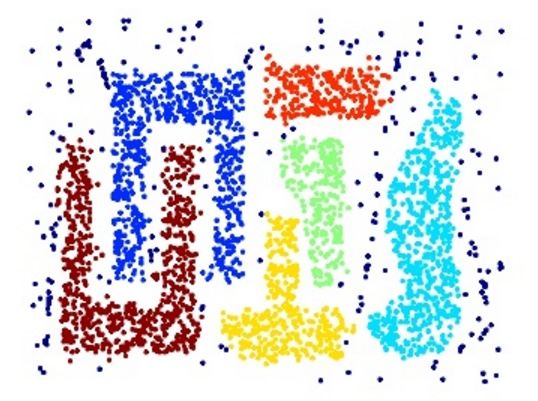
\includegraphics[width=10cm]{dbscan_nonspheric.jpg}
  \caption{Zes niet-sferische clusters met ruispunten (donkerblauw) bekomen door DBScan.}
  \label{fig:dbscan_nonspheric}
 \end{figure}

\subsection{Densiteit}
Er zijn verschillende manieren om densiteit te definiëren, wij zullen ons beperken
tot een manier die gebaseerd is op centers.
\begin{definition}
De \textbf{densiteit} (of dichtheid) van een datapunt wordt gegeven door het
aantal datapunten dat binnen een bepaalde straal ($\epsilon$) van het gegeven punt ligt.
\end{definition}

Het is duidelijk dat de dichtheid van een punt zal afhangen van de keuze van de
straal. De definitie van dichtheid laat ons toe om punten te classificeren in drie 
categorieën:
\begin{itemize}
	\item \textbf{Kernpunten:} Dit zijn punten die middenin een cluster liggen,
	bekomen door een dicht\-heidsgebaseerd algoritme.	Een punt wordt een kernpunt
	genoemd als de dichtheid een bepaalde waarde (density-treshold)
	overschrijdt, deze waarde wordt op voorhand gespecificeerd.
	
	\item \textbf{Randpunten:} Deze punten liggen op de rand van een cluster.
	Ze behoren niet tot de categorie van kernpunten maar liggen wel in de
	omgeving van een kernpunt.

	\item \textbf{Ruispunten:} Elk punt dat niet behoort tot één van
	bovenstaande categorieën noemt men een ruispunt (noise point).
\end{itemize}

\subsection{Algoritme}
Het DBScan algoritme werkt als volgt: elk paar kernpunten $(x,y)$ die dicht genoeg bij elkaar liggen (dist$(x,y)\leq \epsilon$) worden in dezelfde cluster
gestoken. Randpunten zullen op dezelfde manier behoren tot de cluster van een kernpunt. Ruispunten worden genegeerd.

\begin{opm}
Het kan gebeuren dat randpunten tot verschillende clusters kan behoren, in dat geval moet men een beslissing maken tot welke cluster het punt moet behoren.
\end{opm}

\begin{algorithm}
\caption{DBScan}\label{dbscan}
\textbf{Input:} een verzameling $\{x_1, \ldots, x_n\}$ $d$-dimensionale datapunten, een straal $\epsilon$ en een density-treshold $MinPts$.\\
\textbf{Output:} een verzameling $\{c_1, \ldots, c_k\}$ clusters.
\begin{algorithmic}[1]
\State Geef elk datapunt een label (kern-, rand-, ruispunt).
\State Verwijder de ruispunten.
\State Verbind alle kernpunten die voldoende dicht (afstand $<\epsilon$) bij elkaar liggen.
\State Maak een cluster van elke verzameling kernpunten die verbonden zijn.
\State Voeg elk randpunt toe aan (één van) de cluster(s) van zijn bijhorende kernpunten.
\end{algorithmic}
\end{algorithm}

\subsubsection{Bepalen van parameters $\epsilon$ en $MinPts$}
Er bestaat in het algemeen geen optimale manier om de parameters $\epsilon$ en $MinPts$
te schatten. In sommige gevallen kan men de parameters bepalen uit de betekenis
van de data. Zo kan bijvoorbeeld $\epsilon$ een fysieke afstand voorstellen en $MinPts$
het gewenste minimum aantal punten in een cluster. \footnote{In het algemeen kan
een cluster bestaan uit minder dan $MinPts$ datapunten. Een kernpunt dat enkel
omgeven is door randpunten vormt een cluster op zich. De randpunten kunnen ook
randpunten zijn van andere clusters en om bepaalde redenen tot die clusters worden
opgenomen zodat de cluster, gevormd door het kernpunt, bestaat uit slechts één punt.}

Een vuistregel voor het schatten van de parameter $MinPts$ wordt gegeven door
$MinPts \geq d+1$ waarbij $d$ de dimensie is van de data. Wanneer $MinPts \leq 2$
zal het resultaat hetzelfde zijn als bij een hiërarchische clustering waarbij men
de partitie met $\epsilon$ clusters beschouwt. Om deze reden wordt $MinPts \geq 3$
gekozen. Hogere waarden gaan beter om met ruis en leiden in het algemeen tot
significantere clusters. In het algemeen wordt een hogere waarde voor
$MinPts$ gekozen wanneer de dataset groter wordt.

Om $\epsilon$ te schatten, wordt gebruik gemaakt van de bekomen schatter voor
$MinPts (=k)$. Er wordt een $k$-dist plot (Figuur~\ref{kdist}) gemaakt van de data.
Dit is een plot van de afstand tot de $k$-de buur ($k$-distance) in functie van
het aantal datapunten die $k$ buren hebben voor die afstand. Een sterke stijging
van deze grafiek wijst op het feit dat vermoedelijk alle dense gebieden reeds zijn
beschouwd. Punten die niet tot een cluster behoren zullen een hoge $k$-dist hebben.
De $k$-dist waarvoor de grafiek een sterke stijging vertoont, is dus een goede
kandidaat voor $\epsilon$. Het is duidelijk dat wanneer men deze waarde neemt voor
$\epsilon$, alle punten die een $k$-dist hebben kleiner dan $\epsilon$ kernpunten
zullen zijn. De andere datapunten zullen dan rand- of ruispunten zijn.

 \begin{figure}[!ht]\centering
  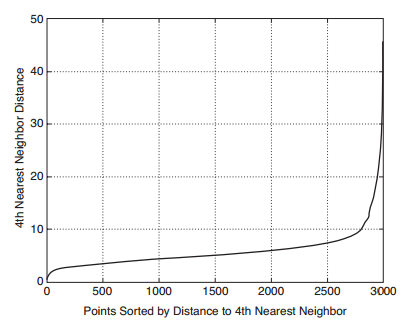
\includegraphics[width=10cm]{dbscan_kdist.png}
  \caption{k-distance plot voor clusters van gelijke densiteit,\\$10$ is de schatting voor $\epsilon$.}
  \label{kdist}
 \end{figure}
\newpage
\subsubsection{Clusters met verschillende densiteit}
Zolang de clusters gelijkaardige densiteit hebben zal het algoritme over het algemeen
goed presteren. Wanneer de clusters echter een zeer verschillende densiteit hebben,
zal het moeilijk zijn om geschikte schatters te vinden voor de parameters. We leggen
dit uit a.d.h.v. een voorbeeld.
\begin{vb}
In Figuur~\ref{dbscan_density} zien we $4$ clusters $A, B, C$ en $D$. De densiteit
(hoe donkerder het gebied, hoe hoger de densiteit) van $A$ en $B$ zijn echter 
verschillend van de densiteit van clusters $C$ en $D$.
Wanneer we de parameters willen schatten m.b.v. de $k$-dist plot, zullen er duidelijk
twee stijgingen zichtbaar zijn. Een eerste stijging zal zichtbaar zijn
vanaf het aantal punten in clusters $A$ en $B$ bereikt is. De tweede stijging zal
zichtbaar zijn vanaf het aantal
punten in de linkerhelft (inclusief ruispunten) opgeteld bij het aantal
punten van clusters $C$ en $D$ bereikt is. Wanneer men de schatter voor $\epsilon$ bekomt door
de $k$-dist bij de eerste stijging te nemen, zullen clusters $C$ en $D$ ook als
ruis beschouwd worden, men bekomt twee clusters nl. $A$ en $B$. In het geval dat de $k$-dist bij de tweede
stijging gebruikt wordt, zullen de clusters $A$ en $B$ niet van elkaar
en de omliggende ruis kunnen onderscheiden worden, men bekomt $3$ clusters
nl. $C$, $D$ en de volledige linkerhelft.
 \begin{figure}[!ht]
  \centering
  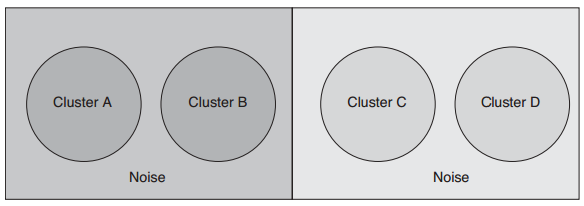
\includegraphics[width=15cm]{dbscan_density.png}
  \caption{DBScan met verschillende densiteit, in zo'n situatie zal het algoritme
  niet in staat zijn de vier clusters te onderscheiden.}
  \label{dbscan_density}
 \end{figure}
\end{vb}





\newpage
\section{Clusterevaluatie}
\label{sec:eval}
Omdat er zo veel verschillende methoden zijn om data te clusteren en ze niet
allemaal gelijke resultaten opleveren, is het belangrijk dat we in staat zijn
om clusters te evalueren. Aangezien het resultaat van bepaalde algoritmen een
clustering is die afhangt van de (al dan niet willekeurig) gekozen beginsituatie, 
willen we ook clusteringen bekomen door hetzelfde algoritme met verschillende
beginsituaties te vergelijken.
Een voorbeeld hiervan is het $k$-means algoritme uit Sectie~\ref{sec_kmeans}.
We hebben gezien dat men vaak het $k$-means algoritme meermaals uitvoerd
op dezelfde data maar met andere beginsituaties. Men kan dan gebruik maken
van de SSE om te bepalen welk van alle clusteringen een beter resultaat oplevert.
Het is duidelijk dat het minimaliseren van de SSE niet bij elke soort clusteringen
van toepassing is, bij het DBScan-algoritme uit Sectie~\ref{sec_dbscan} zal dit in het algemeen niet werken.

In het geval dat er geen sprake is van clusters (bijvoorbeeld uniform verdeelde
punten) zullen de besproken algoritmen toch clusters vormen, ook dit is een reden
waarom clusterevaluatie wel degelijk belangrijk is. Wanneer de data zich bevinden
in een laag (dim $\leq 3$) dimensionale ruimte, kan men vaak op het oog zien of
een clustering een goede clustering is. Wanneer men echter data in een hogere
dimensie beschouwt wordt dit veel moeilijker.

Op basis van de gebruikte informatie onderscheiden we twee klassen evaluatiemethodes:

\begin{itemize}
 \item[(i)] Methoden die geen gebruik maken van externe informatie noemen we
 \textbf{unsupervised}. Men kan eenerzijds meten hoe nauw de data in een cluster
 aan elkaar verwant zijn (cluster cohesie) en anderzijds hoe sterk clusters van elkaar
 verschillen (cluster separation of isolation).
 \item[(ii)] Methoden die wel gebruik maken van externe informatie om clusters te evalueren
 noemen we \textbf{supervised}. Vaak komt dit neer op het vergelijken van een bekomen
 clustering met een onderliggende structuur op de data die reeds bekend was.
 Men kan bijvoorbeeld de cluster labels vergelijken met labels van een andere
 classificatie (entropy-based cluster validation).
\end{itemize}

Anderzijds onderscheiden we methodes die clusters individueel vergelijken en relatieve
me\-thodes. Relatieve methodes vergelijken meerdere clusteringen met elkaar.
Het vergelijken van de SSE tussen verschillende clusteringen is een voorbeeld van een 
relatieve unsupervised methode.

\subsection{Cohesie en separatie}
Veel unsupervised clusterevaluatiemethodes voor
paritionele clusteringen maken gebruik van cohesie en separatie van clusters.
In het algemeen kan een maat voor de geldigheid van een clustering als volgt
gedefinieerd worden:
$$validity = \sum\limits_{i=1}^kw_i\hspace{1mm} validity(C_i).$$

Waarbij $k$ het aantal clusters is,
$validity(C_i)$
\footnote{De geldigheidsfunctie $validity(C_i)$ kan afhangen van meerdere
clusters in het algemeen, bijvoorbeeld bij separatie in het geval van
graaf-gebaseerde clusters.} een maat is voor de geldigheid van de cluster $C_i$ en 
$w_i$ een gewicht. De gewichten kunnen bijvoorbeeld afhangen van de grootte van
cluster. De geldigheid van een cluster kan de cohesie of de separatie zijn of een
functie die beide combineert.
Als de geldigheidsfunctie de cohesie is, dan stemt een lage waarde overeen
met een goede cluster (de elementen in de cluster liggen dicht bijeen).
In het geval van separatie is dit net omgekeerd (de elementen in een cluster liggen
ver van de elementen van andere clusters).

We bespreken nu enkele voorbeelden van geldigheidsfuncties.

\subsubsection*{Graaf-gebaseerde clusters}
Wanneer data in de vorm van een gewogen, complete graaf wordt voorgesteld
en clusters klieken (complete componenten) zijn, dan kan men de geldigheidsfuncties
van clusters als volgt definiëren:
\begin{align*}
cohesion(C_i) &= \sum\limits_{x\in C_i, y\in C_i} d(x,y),\\
separation(C_i, C_j) &= \sum\limits_{x\in C_i, y\in C_j} d(x,y),
\end{align*}
met $d(x,y)$ het gewicht tussen top $x$ en $y$.

\subsubsection*{Prototype-gebaseerde clusters}
Wanneer de dataset zeer groot is, dan vergen vorige formules zeer veel rekenwerk.
Bij prototype-gebaseerde clusters kan dit eenvoudig voorkomen worden
door gebruik te maken van de centers van de clusters.
Mogelijke geldigheidsfuncties zijn dan:
\begin{align*}
cohesion(C_i) &= \sum\limits_{x\in C_i} d(x,c_i),\\
separation(C_i) &= d(c_i,c),\\
separation(C_i, C_j) &= d(c_i,c_j),
\end{align*}
met $c_i$ het center van cluster $C_i$ en $c$ het center van alle data.
\newline

Een typische manier om de separatie van clusters te meten wanneer
de afstand tussen punten gegeven wordt door de Euclidische afstand is de
SSB (Eng: between group sum of squares). Dit is de
som van de kwadratische afstanden tussen de de centers van de clusters $c_i$ ($i=1,\ldots ,k$)
en het center van alle data $c$.
De totale SSB van een clustering wordt gegeven door de som van
de SSB's van de $k$ clusters:
$$\TSSB = \sum\limits_{i=1}^km_id(c_i,c)^2.$$
In eigenschap~\ref{eign} (ii) zien we dat in het speciaal geval van gelijke clustergroottes ($m_i = \dfrac{m}{k}\quad \forall i \in \{1,2,\ldots,k\}$),
de $\TSSB$ ook d.m.v. paarsgewijze afstanden (tussen clustercenters) kan gedefinieerd worden.
\newline

We tonen nu enkele interessante eigenschappen aan die verbanden leggen tussen graaf-gebaseerde
en prototype-gebaseerde clusteringen (i) en tussen cohesie en adhesie in 
specifieke gevallen (iii). Alle eigenschappen maken gebruik van volgend lemma.

\begin{lem} Voor een cluster $C_i$ geldt:
  $\sum\limits_{x\in C_i}\sum\limits_{y\in C_i}(x-c_i)(y-c_i) = 0.$
\end{lem}

\begin{proof}
 
 \begin{align*}
  \sum\limits_{x\in C_i}\sum\limits_{y\in C_i}(x-c_i)(y-c_i)
  &= \sum\limits_{x\in C_i}\sum\limits_{y\in C_i}(-xc_i - yc_i + c_i^2 + xy)\\
  &= -c_i\sum\limits_{x\in C_i}\sum\limits_{y\in C_i}(x+y) + c_i^2\sum\limits_{x\in C_i}\sum\limits_{y\in C_i}1 + (\sum\limits_{x\in C_i}x)(\sum\limits_{y\in C_i}y)\\
  &= - c_i2m_i^2c_i + c_i^2m_i^2 + m_i^2c_i^2\\ &= 0\\
 \end{align*}
\end{proof}


\begin{eign}\ \\
 \label{eign}
 \begin{itemize}
  \item[(i)] $\CSSE =\sum\limits_{x\in C_i}d(c_i,x)^2 
  = \dfrac{1}{2m_i}\sum\limits_{x\in C_i}\sum\limits_{y\in C_i}d(x,y)^2.$
  \item[(ii)] $\TSSB = \sum\limits_{i=1}^k\dfrac{m}{k}d(c_i,c)^2 = 
  \dfrac{1}{2k}\sum\limits_{i=1}^k\sum\limits_{j=1}^k\dfrac{m}{k}d(c_i,c_j)^2.$
  \item[(iii)] $\TSS = \sum\limits_{i=1}^k\sum\limits_{x\in C_i}(x-c)^2=
  \SSE + \SSB$
 \end{itemize}
\end{eign}




\begin{proof}
We tonen bovenstaande eigenschappen voor het eendimensionaal geval aan,
de bewijzen van de eigenschappen verlopen analoog.
 \begin{itemize}

  \item[(i)]
  \begin{align*}
  &\dfrac{1}{2m_i}\sum\limits_{x\in C_i}\sum\limits_{y\in C_i}(x-y)^2\\
  &= \dfrac{1}{2m_i}\sum\limits_{x\in C_i}\sum\limits_{y\in C_i}((x-c_i) - (y-c_i))^2\\
  &= \dfrac{1}{2m_i}\left(\sum\limits_{x\in C_i}\sum\limits_{y\in C_i}(x-c_i)^2+\sum\limits_{x\in C_i}\sum\limits_{y\in C_i}(y-c_i)^2-2\sum\limits_{x\in C_i}\sum\limits_{y\in C_i}(x-c_i)(y-c_i)		  \right)\\
  &= \dfrac{1}{2m_i}\left(\sum\limits_{x\in C_i}\sum\limits_{y\in C_i}(x-c_i)^2+\sum\limits_{x\in C_i}\sum\limits_{y\in C_i}(y-c_i)^2\right)\\
  &= \dfrac{1}{m_i}\sum\limits_{x\in C_i}m_i(x-c_i)^2\\
  &= \sum\limits_{x\in C_i}(x-c_i)^2\\
  &= \SSE
  \end{align*}

  \item[(ii)]
  \begin{align*}
  &\dfrac{1}{2k}\sum\limits_{i=1}^k\sum\limits_{j=1}^k\dfrac{m}{k}(c_j-c_i)^2\\
  &= \dfrac{1}{2k}\sum\limits_{i=1}^k\sum\limits_{j=1}^k\dfrac{m}{k}((c-c_i)-(c-c_j))^2\\
  &= \dfrac{1}{2k}\left(\sum\limits_{i=1}^k\sum\limits_{j=1}^k\dfrac{m}{k}(c-c_i)^2 + \sum\limits_{i=1}^k\sum\limits_{j=1}^k\dfrac{m}{k}(c-c_j)^2
  - 2\sum\limits_{i=1}^k\sum\limits_{j=1}^k\dfrac{m}{k}(c-c_i)(c-c_j)\right)\\
  &= \dfrac{1}{2k}\left(\sum\limits_{i=1}^k\sum\limits_{j=1}^k\dfrac{m}{k}(c-c_i)^2 + \sum\limits_{i=1}^k\sum\limits_{j=1}^k\dfrac{m}{k}(c-c_j)^2\right)\\
  &= \dfrac{1}{k}\sum\limits_{i=1}^km(c-c_i)^2\\
  &= \SSB
  \end{align*}
  \item[(iii)]
  \begin{align*}
  \TSS &= \sum\limits_{i=1}^k\sum\limits_{x\in C_i}(x-c)^2\\
  &= \sum\limits_{i=1}^k\sum\limits_{x\in C_i}((x-c_i)-(c-c_i))^2\\
  &= \sum\limits_{i=1}^k\sum\limits_{x\in C_i}(x-c_i)^2+\sum\limits_{i=1}^k\sum\limits_{x\in C_i}(c_i-c)^2 - 2\sum\limits_{i=1}^k\sum\limits_{x\in C_i}(x-c_i)(c-c_i)\\
  &= \sum\limits_{i=1}^k\sum\limits_{x\in C_i}(x-c_i)^2+\sum\limits_{i=1}^k\sum\limits_{x\in C_i}(c_i-c)^2\\
  &= \sum\limits_{i=1}^k\sum\limits_{x\in C_i}(x-c_i)^2+\sum\limits_{i=1}^km_i(c_i-c)^2\\
  &= \SSE + \SSB
  \end{align*}
 \end{itemize}
\end{proof}





\begin{opm}
 In de derde eigenschap zien we dat de som van de SSE en SSB een constante is
 (TSS, total sum of squares). Het minimaliseren van de SSE (cohesie) is dus equivalent
 aan het maximaliseren van de SSB (separatie).
\end{opm}



\subsubsection*{Gewichten}
De gewichten die gebruikt worden voor de geldigheidsmaten kunnen erg verschillen,
vaak zullen ze echter gerelateerd zijn aan de grootte van de clusters.
In tabel~\ref{clustervaltable} zien we een aantal veelgebruikte gewichten en
geldigheidsfuncties.

\begin{table}[!ht]
\begin{tabular}[!ht]{|C|C|c|}
\hline
\text{cluster geldigheidsfunctie}&\text{cluster gewicht}&type\\
\hline
\hline
\sum\limits_{x\in C_i, y\in C_i} d(x,y)&\dfrac{1}{m_i}&graaf-gebaseerd, cohesie\\
\hline
\sum\limits_{x\in C_i} d(x,c_i)&1&prototype-gebaseerd, cohesie\\
\hline
d(c_i,c)&m_i&prototype-gebaseerd, separatie\\
\hline
\sum\limits_{j=1, j\neq i}^k\sum\limits_{x\in C_i, y\in C_j} d(x,y)
&\dfrac{1}{\sum\limits_{x\in C_i, y\in C_i} d(x,y)}&graaf-gebaseerd, cohesie en separatie\\
\hline
\end{tabular}
\caption{Enkele veelgebruikte cluster geldigheidsfuncties met bijhorende gewichten.\\ De elementen in de eerste kolom zijn 
functies die de geldigheid van een cluster $C_i$ meten, in de tweede kolom
staan gewichten die horen bij deze maten. In de laatste kolom zien we voor
welke soorten clusteringen de functies kunnen gebruikt worden en wordt ook
het type geldigheidsfunctie gegeven.
Hierbij is $m_i$ de grootte van cluster $C_i$ en $k$ het aantal clusters.}
\label{clustervaltable}
\end{table}

\begin{opm}
 Elke unsupervised geldigheidsmaat kan gebruikt worden als doelfunctie
 voor een clusteringsalgoritme en omgekeerd. We gebruikten de geldigheidsmaten
 om een volledige clustering te evalueren. We kunen echter ook de clusters individueel
 evalueren op basis van deze maten. Vervolgens kunnen de clusters geordend
 worden volgens geldigheid. Als in een bekomen clustering
 bepaalde clusters een zeer lage cohesie hebben ten opzichte van andere,
 dan kunnen de clusters met lage cohesie opgesplitst worden in
 subclusters.
\end{opm}




\subsubsection*{De silhouettecoëfficiënt}

De bijdrage van een datapunt ($x \in C_i$) aan de geldigheid van een cluster kan
bepaald worden. Hiervoor wordt bijvoorbeeld gebruik gemaakt van de silhouettecoëfficiënt die als volgt berekend wordt:
\begin{enumerate}
 \item Bereken de gemiddelde afstand van $x$ tot alle andere datapunten
 van de cluster $C_i$:\\ $a_x:=\frac{1}{m_i-1}\sum\limits_{y\in C_i\setminus\{x\}}d(x,y).$
 \item Bepaal het minimum van de som van de gemiddelde afstanden van $x$ tot alle punten
 van een andere cluster:\\
 $b_x:=\min\limits_{j\neq i}\left(\frac{1}{m_j}\sum\limits_{y\in C_j}d(x,y)\right).$
 \item De silhouettecoëfficiënt voor $x$ wordt gegeven door:
 $s_x = \dfrac{b_x-a_x}{\max(a_x,b_x)}.$
\end{enumerate}

Per definitie geldt $|s_x|\leq1$, een negatieve waarde voor de silhouettecoëfficiënt slaat echter op het feit dat de gemiddelde afstand van $x$ tot
de andere punten in zijn cluster hoger is dan de minimale gemiddelde afstand
tot punten van een andere cluster en dat is natuurlijk ongewenst.
Een negatieve silhouettecoëfficiënt zal echter zelden voorkomen
omdat de meeste clusteringsalgoritmen dit impliciet vermijden. Als $a_x<b_x$, dan
geldt dat $s_x = 1- a_x/b_x$, dit nadert naar
$1$ wanneer $a_x$ afneemt of $b_x$ toeneemt. Het afnemen van $a_x$
wijst erop dat $x$ dicht bij de andere datapunten in de cluster ligt.
Het toenemen van $b_x$ slaat op het feit dat $x$ ver van alle andere
clusters ligt. We wensen dus een silhouettecoëfficiënt te verkrijgen
dicht bij $1$.

Voor de evaluatie van een cluster, kan de gemiddelde silhouettecoëfficiënt
van zijn punten bepaald worden als geldigheidsfunctie. Voor
een volledige clustering kan de gemiddelde silhouettecoëfficiënt
van alle datapunten berekend worden.

\subsection{Gelijkheidsmatrix}
In Sectie~\ref{sec_proxmat} definieerden we een gelijkheidsmatrix, een $n\times n$- matrix die de gelijkheid tussen datapunten voorstelt.
Men kan hiervan gebruikmaken om clusteringen te evalueren door ener\-zijds deze matrix te vergelijken met een ideale variant (d.m.v. correlatie) en anderzijds
door de afstanden visueel voor te stellen.

\subsubsection*{Correlatie}
In een ideale clustering zijn de elementen in clusters sterk gelijkend aan elkaar,
maar erg verschillend van elementen in andere clusters. Dit stemt overeen met een
gelijkheid van $1$ voor punten in dezelfde cluster en een gelijkheid van $0$ voor
punten uit verschillende clusters. Als men nu de rijen (en kolommen) van de
gelijkheidsmatrix zodanig permuteert dat de elementen uit dezelfde clusters
gegroepeerd worden, krijgen we een blokdiagonaalmatrix.
De ideale gelijk\-heidsmatrix bestaat dus uit vierkante blokken met waarde $1$ op de diagonaal en $0$ elders.
De kwaliteit van een clustering kan dan bepaald worden door de correlatie te berekenen tussen de ideale gelijkheidsmatrix en de effectieve gelijkheidsmatrix die overeenstemt met de data.
Wanneer de matrices sterk gecorreleerd zijn (correlatie $\approx 1$) kan men besluiten dat de gevormde clusters bestaan uit sterk op elkaar gelijkende datapunten
en dat de clusters onderling zeer verschillend zijn.
Men kan dit ook visualiseren door de aangepaste gelijkheidsmatrix (waarbij de rijen en kolommen per cluster gegroepeerd staan) te plotten.

\begin{opm}
 Het bepalen van de correlatie is rekenintensief, daarom wordt vaak gekozen om slechts
 een sample van de data te gebruiken om de correlatie te benaderen.
\end{opm}



\subsubsection*{Hiërarchische clusteringen}
Bovenstaande methodes zijn vooral gericht op partitionele clusteringsalgoritmen, voor hiërarchisch geclusterde data bestaat er een gelijksoortige aanpak die gebruik maakt van de
`cophenetic distance'. De cophenetic distance tussen twee datapunten wordt gegeven door de afstand tussen de twee clusters waartoe de punten behoren wanneer die twee clusters
worden samengevoegd in het agglomeratieve hiërarchisch clusteringsalgoritme. De cophenetic distance matrix wordt gegeven door de symmetrische matrix met als elementen
de cophenetic distance tussen elk paar datapunten.
Om de kwaliteit van een clustering te testen, bepaalt men de `cophenetic correlation coeffiient' (CPCC). Dit is de correlatie tussen de cophenetic distance matrix en de afstandsmatrix
van de data. Een hoge correlatie wijst op een goede clustering. Deze correlatie\-coëfficiënt wordt voornamelijk gebruikt om verschillende hiërarchische clusteringsalgoritmen met elkaar te vergelijken.

\subsection{Bepalen van het aantal clusters}
Een cruciale stap in het clusteren van data is het bepalen van het aantal clusters. In sommige gevallen kan men al op voorhand weten hoeveel clusters te verwachten zijn
door externe informatie of een visualisatie van de data. Dit is echter niet altijd het geval, een meer algemene aanpak is door een grafiek te  maken van de maat van evaluatie
in functie van het aantal clusters. Voor (agglomeratieve) hiërarchische clusteringsalgoritmen vereist deze aanpak niet veel extra rekenwerk omdat men stapsgewijs van $n$ clusters
naar één cluster gaat. In het geval van partitionele clusteringsalgoritmen zal men meerdere keren het algoritme moeten uitvoeren voor verschillende clusteraantallen wat zijn impact
heeft op de snelheid van het proces. Men kan kiezen om de SSE en de silhouettecoëfficiënt te plotten in functie van het aantal clusters. Wanneer de SSE amper verlaagt naarmate het aantal clusters stijgt, zal een hoger aantal clusters veelal nutteloos blijken. In de grafiek van de silhouettecoëfficiënt wijst een piek op een goed aantal clusters. Een combinatie van beide plots
wordt vaak gebruikt om het ideale aantal clusters voor een $k$-means algoritme te bepalen.

\subsection{Geschikt voor clustering}
We kunnen nu data clusteren, een clustering evalueren en bepalen hoeveel clusters er moeten gevormd worden, maar dit alles is overbodig als blijkt dat de data totaal niet geschikt is om te clusteren. Men kan verschillende algoritmen loslaten op data en kijken of er kwalitatieve clusters gevormd worden, maar in het geval dat alle clusteringen slechts weinig kwalitatief zijn,
zal er veel rekenwerk gespendeerd zijn zonder enig resultaat. Men kan dit in sommige gevallen voorkomen door te kijken of er redenen zijn om te geloven dat de data geschikt is om te clusteren.
Een mogelijke methode om dit te doen is door de `Hopkins statistiek' te bepalen.

\newpage
\begin{definition}
Beschouw $p$ datapunten willekeurig te kiezen uit het universum en een sample van $p$ datapunten uit de geobserveerde data.
Bepaal de afstand van de punten tot hun dichtste buur uit de geobserveerde data, noem de bekomen afstanden voor de $p$ willekeurige datapunten $\{u_1, u_2, \ldots, u_p\}$  en voor
de datapunten uit de sample $\{w_1, w_2, \ldots, w_p\}$ . De Hopkinsstatistiek wordt gegeven door:
$$H = \dfrac{\sum\limits_{i=1}^pw_i}{\sum\limits_{i=1}^pu_i + \sum\limits_{i=1}^pw_i}.$$
Als $H\approx1$, dan is er een indicatie dat de data geclusterd kan worden.
Als de datapunten uniform verdeeld zijn verwachten we dat $H\approx0.5$.
\end{definition}



\newpage
\setcounter{section}{0}
\renewcommand{\thesection}{\Alph{section}}
\section{Appendix}
\subsection{Stirling getallen van de tweede soort}
\label{stirling}
Het aantal mogelijke partities met $k$ elementen van een verzameling met $n$ elementen wordt gegeven door
de Stirling getallen van de tweede soort $S(n,k)$.
We bepalen een recursieve manier om $S(n,k)$ te berekenen.
Eerst merken we volgende triviale gelijkheden op:
\begin{itemize}
	\item $S(n,1) = 1$
	\item $S(n,n) = 1$
	\item $S(n,k) = 0$ \quad als $k>n$.
\end{itemize}
Veronderstel dat alle mogelijke partities van een verzameling met $n-1$ elementen gekend zijn.
We willen $S(n,k)$ berekenen, hiervoor maken we gebruik van $S(n-1,k-1)$ en $S(n-1,k)$ (gekend wegens de inductiehypothese).
Een partitie van $n$ objecten in $k$ verzamelingen kan nu gevormd worden op twee manieren:
\begin{enumerate}
	\item het $n$-de element wordt toegevoegd als singleton bij een partitie van $n-1$ elementen in $k-1$ verzamelingen (één keuze),
	\item het $n$-de element wordt toegevoegd in één van de $k$ verzamelingen van een partitie van  $n-1$ elementen in $k$ verzamelingen ($k$ keuzes).
\end{enumerate} 
De recursie wordt dus gegeven door:
$$S(n,k) = S(n-1,k-1) + k\cdot S(n-1,k).$$
Het is duidelijk dat men hiermee $S(n,k)$ recursief kan berekenen voor alle waarden $k\in \mathbb{N}$ en $n\in \mathbb{N}$.
De Stirling getallen van de tweede soort kunnen ook expliciet berekend worden als volgt:
$$S(n,k) = \dfrac{1}{k!}\sum\limits_{j=0}^k(-1)^j\binom{k}{j}(k-j)^n.$$


\newpage
\bibliography{bachelorproef}{}
\nocite{jain1988algorithms}
\nocite{wiki}
\bibliographystyle{plain}
\end{document}
